\clearpage
\section{Soft- und Firmware}\label{sec:Soft-undFirmware}


Im folgenden Abschnitt werden Anforderungen, Konzept und die Umsetzung der Software dokumentiert. Die Lösungsfindung und ihre Prozess wird nachfolgend beschrieben. 

\subsection{Anforderungen}\label{subsec:Software_Anforderungen}

Wie bereits im Abschnitt \ref{subsec:VergleichswerteundMessgrössenMesh} wurden die Anforderungen in der Aufgabenstellung (siehe Anhang \ref{app:Aufgabenstellung}) sowie im Pflichtenheft (siehe Anhang \ref{app:Pflichtenheft}) vorgängig festgelegt. Im Fokus steht das erfassen der wichtigsten Messgrössen welche bereits in Abschnitt \ref{subsec:VergleichswerteundMessgrössenMesh} definiert wurden. 

Die Erfassung der Messwerte muss in allen Mesh-Netzwerken möglich sein. Um die Messresultate vergleichen zu können müssen die gleichen Ausgangslagen vorliegen, sowie die selben Messmethoden angewendet werden. 


\subsection{Konzept}\label{subsec:Software_Konzept}

Das Konzept der Messung wurde in Abschnitt \ref{sec:BenchmarkKonzeptMeshNetzwerke} erläutert. Die Software soll so aufgebaut sein, dass sie von allen Mesh-Stacks genutzt werden kann. Zur Umsetzung der Mesh-Stacks mittles der \textit{NRF-Platform} sind folgende SDKs vorhanden: 

\begin{itemize}
	\item \textit{\textbf{nRF Connect SDK}}: Auf dem Zephyr-RTOS aufbauende SDK. Diese soll in Zukunft alle drei Mesh-Protokolle (Bluetooth-Mesh, Openthread und Zigbee) unterstützen. Wird jedoch noch nicht zum Einsatz in End-Produkten empfohlen. \cite{nordic_semi_welcome_to_the_nrf_connect_sdk_2020}
	\item \textit{\textbf{nRF SDK for Thread and Zigbee}}: Proprietäre SDK Library von Nordic Semiconductor. Thread integration mittels Openthread, Zigbee einbindung mittels ZBOSS. \cite{nordic_semi_nrf_sdk_for_thread_and_zigbee_2020}
	\item \textit{\textbf{nRF SDK for Mesh}}: Proprietäre SDK Library von Nordic Semiconductor für Bluetooth-Mesh. Ist zur Produktion freigegeben. \cite{nordic_semi_nrf_sdk_for_mesh_2020}
\end{itemize}

Die Messungen sollten trotz der verschiedenen Bibliotheken möglichst einheitlich sein, um die Vergleichbarkeit nicht zu beeinträchtigen. Um eine möglichst unabhängig von der verwendeten SDK zu bleiben, wurde auf eine selbst entwickelte Kommunikation im Benchmark Management gesetzt. Dazu wurden  diverse Module der P2P-Testinfrastruktur nachempfunden. 


\subsection{Umsetzung}\label{subsec:Software_Umsetzung}


Die Software und Firmware für die Mesh Benchmarks setzt sich aus diversen Modulen zusammen. Die Tabelle \ref{tab:UebersichtSoftware} zeigt eine Übersicht der wichtigsten Module und deren Verwendung in den 3 Benchmark Teilen: BLE Mesh, Thread und Zigbee.
Gemeinsame Module auf Firmware Ebene sind im Ordner SharedLib im Github Repository\footnotemark\ zusammengefasst.

Jene Python Scripts für das Benchmark Management stehen im gleichnamigen Ordner auf dem Github Repository zur Verfügung.
Die Stack bezogenen Implementationen der Benchmark Firmware werden in den individuellen Teilen \ref{part:BluetoothMesh}, \ref{part:Thread} und \ref{part:Zigbee} behandelt.


%\newcommand{\rotcells}[1]{%
%  \rotatebox[origin=c]{90}{ #1 }%
%}

\begin{table}
\centering
\begin{tabular}{|l|l|l|c|} 
\hline
Library & Funktion & Modul & Referenz \\ 
\hline
\multirow{8}{*}{SharedLib} & Statemachine & bm\_statemachine.c & \ref{subsubsec:StatemachineSoftware} \\ 
\cline{2-4}
 & Timesync & bm\_timesync.c & \ref{subsubsec:Timesync}  \\ 
\cline{2-4}
 & Control & bm\_control.c & \ref{subsubsec:Control} \\ 
\cline{2-4}
 & Report & bm\_report.c & \ref{subsubsec:Report} \\ 
\cline{2-4}
 & Logging & bm\_log.c & \ref{subsubsec:Logging} \\ 
\cline{2-4}
 & Flash Save & bm\_flash\_save.c & \ref{subsubsec:FlashSave} \\ 
\cline{2-4}
 & CLI & bm\_cli.c & \ref{subsubsec:CLI} \\ 
\cline{2-4}
 & Low Layer Radio & bm\_radio.c & \ref{subsubsec:LowLevelRadio} \\ 
 \cline{2-4}
 & \begin{tabular}[c]{@{}l@{}}Random and Sequential \\ Traffic Generator  \end{tabular} & bm\_rand.c & \ref{subsubsec:TrafficGenerator} \\ 
\hline
\multicolumn{1}{l}{} & \multicolumn{1}{l}{} & \multicolumn{1}{l}{} & \multicolumn{1}{l}{} \\ 
\hline
\multirow{4}{*}{\begin{tabular}[c]{@{}l@{}}Benchmark\\Management \end{tabular}} & Flash & Flasher.py & \ref{subsubsec:Flash} \\ 
\cline{2-4}
 & Configurator & Configurator.py & \ref{subsubsec:Configurator} \\ 
\cline{2-4}
 & Benchmark and Reporter & \begin{tabular}[c]{@{}l@{}}Benchmark\_and\_\\Reporter.py \end{tabular} & \ref{subsubsec:BenchmarkandReporter} \\ 
\cline{2-4}
 & Analysis & Analysis.py & \ref{subsubsec:Analysis} \\ 
\hline
\multicolumn{1}{l}{} & \multicolumn{1}{l}{} & \multicolumn{1}{l}{} & \multicolumn{1}{l}{} \\ 
\hline
\multirow{4}{*}{BT Mesh} & Stack Init and Configuration & bm\_blemesh.c & \ref{sec:BTMeshUmsetzungBenchmark} \\ 
\cline{2-4}
& Model Handling & bm\_blemesh\_model\_handler.c & \ref{sec:BTMeshUmsetzungBenchmark} \\ 
\cline{2-4}
 & Stack Configuration & bm\_config.h & \ref{sec:BTMeshUmsetzungBenchmark} \\ 
\hline
\multicolumn{1}{l}{} & \multicolumn{1}{l}{} & \multicolumn{1}{l}{} & \multicolumn{1}{l}{} \\ 
\hline
\multirow{2}{*}{Thread} & Stack-Handling & bm\_ot.c & \ref{sec:ThreadUmsetzungBenchmark} \\ 
\cline{2-4}
 & Stack Configuration & bm\_config.h & \ref{sec:ThreadUmsetzungBenchmark} \\ 
\hline
\multicolumn{1}{l}{} & \multicolumn{1}{l}{} & \multicolumn{1}{l}{} & \multicolumn{1}{l}{} \\ 
\hline
\multirow{2}{*}{Zigbee} & Stack Handling & bm\_zigbee.c & \ref{subsubsec:ZigbeeStackHandling} \\ 
\cline{2-4}
 & Stack Configuration & bm\_config.h & \ref{subsubsec:ZigbeeStackConfiguration} \\
\hline
\end{tabular}
\caption{Übersicht Shared Lib und Benchmark Management Module}
\label{tab:UebersichtSoftware}
\end{table}


Sämtliche Firm- und Software Komponenten die für Mesh Benchmark sowie die P2P Testinfrastruktur nötig sind, können auf dem Github Repository zum Projekt unter folgendem \href{https://github.com/Rouben94/P6_Software}{Link\footnotemark[\value{footnote}]}  eingesehen werden. Die nächsten Abschnitte behandeln die Umsetzung der Software, welche von allen Mesh-Stacks genutzt wird.

\footnotetext{\url{https://github.com/Rouben94/P6_Software} \cite{anklin_bobst_horath_rouben94p6_software_nodate}}

\subsection{Shared Library}\label{subsec:SharedLibrary}

Die \textit{Shared Library} ist die geteilte Bibliothek zwischen allen Mesh-Stacks. Sie beherbergt alle relevanten Module um eine Messung zu Verwalten. Der jeweilige Mesh-Stack ist lediglich für das senden und empfangen von Nachrichten, sowie zum Erfassen der Messdaten zuständig. 


\begin{figure}[H]
	\centering
	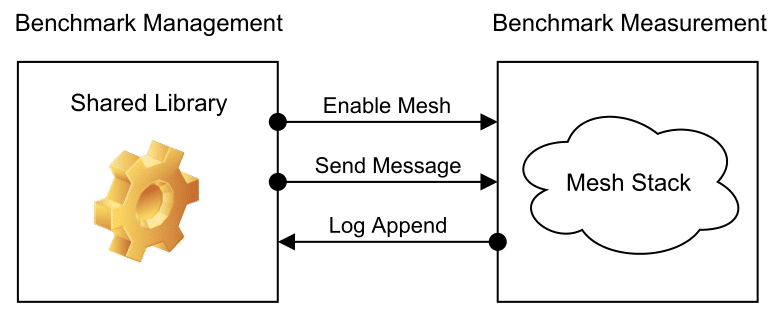
\includegraphics[width=0.6\textwidth]{Shared_Lib_Concept.png}
	\caption{Vereinfachte Anbindung der \textit{Shared Library} an die Mesh-Stacks}\label{fig:ShardeLibConcept}
\end{figure}

Abbildung \ref{fig:ShardeLibConcept} zeigt die vereinfachten Schnittstellen zwischen der Shared-Library und den Mesh-Stacks. Die Bibliothek ist spezifisch für die nRF52840 SOCs zugeschnitten. Um einfach in die jeweilige SDK integrierbar zu sein müssen die Module der Shared-Lib möglichst ohne weitere Abhängigkeiten klar kommen. Sofern Treiber oder externe Bibliotheken für Module benötigt werden, müssen diese von allen SDKs vergleichbar zur Verfügung gestellt werden. Im folgenden Abschnitt wird auf die einzelnen Module der \textit{Shared-Lib} eingegangen. 


\subsubsection{Statemachine}\label{subsubsec:StatemachineSoftware}

Die Statemachine dient dazu den Ablauf, welcher in Abschnitt \ref{subsec:AblaufMesh} beschrieben wurde abzuarbeiten. Sowohl der Master, die Server und Clients arbeiten den in Abbildung \ref{fig:StatemachineFLowgraph} dargestellten Ablauf ab. 

\begin{figure}[H]
	\centering
	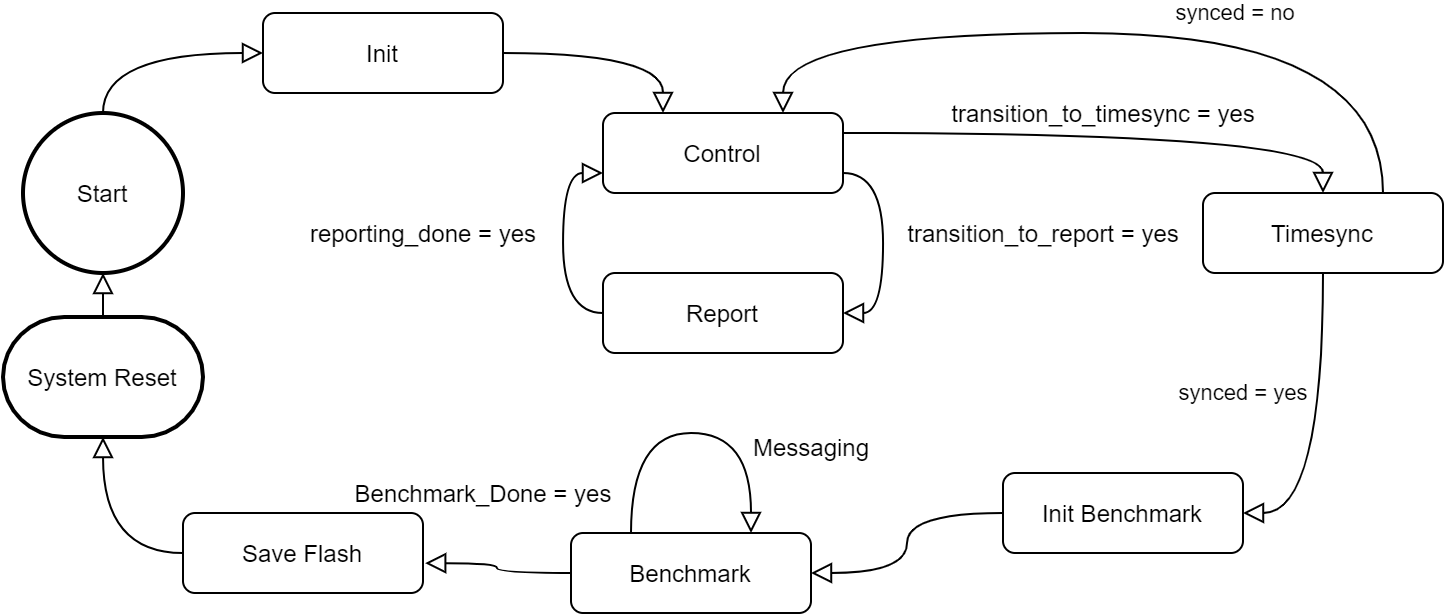
\includegraphics[width=1.0\textwidth]{Statemachine_Flowgraph.png}
	\caption{Flowgraph der Statemachine}\label{fig:StatemachineFLowgraph}
\end{figure}


Die Funktion der Schritte wird im Folgenden grob beschrieben. Zur genauen Untersuchung ist der Source Code unter \cite{rouben94_sharedlib_software_git_2020} verfügbar.

\begin{itemize}
	\item \textbf{\textit{Init:}} Dieser Schritt initialisiert alle notwendige Funktionen (Radio, Timers, usw.). Ebenfalls rekonstruiert er die \textit{Log-Daten} indem er diese aus dem Flash in das RAM kopiert. Nach der erfolgreichen Initialisierung wechselt die Statemachine in den Control-State.
	\item \textbf{\textit{Control:}} Im Control-State wartet jeder Teilnehmer auf eingehende Befehle des Benutzers. Der Master erhält über das Command Line Interface (CLI) den auszuführenden Befehl. Diesen wandelt der Master in eine Nachricht (Control-Message) um und leitet sie über das Radio-Interface an die Slaves weiter.  Alle Slaves (Clients und Servers) erwarten eine Control-Message über das Radio-Interface. Damit alle Clients und Servers die Nachricht empfangen können wiederholt jeder Slave jede Control-Message. Somit wird die Mesh-Fähigkeit der Verwaltungsschicht (Benchmark Managment) sichergestellt. Folgende Transitionen sind vom Control-State zugelassen: 
	\begin{itemize}
		\item \textit{\textbf{Transition to Timesync}}: Wird ein Benchmark gestartet erfolgt dies durch einen Wechsel in den Timesync-State. Jeder Teilnehmer wechselt nach wiederholen der Nachricht in den entsprechenden Schritt. 
		\item \textit{\textbf{Transition to Report}}: Das Reporting wird über den Report-State abgehandelt. Nur der Teilnehmer von welchem Reports angefordert wurden, wechselt in den Report-State. 
	\end{itemize} 	
	\item \textbf{\textit{Timesync:}} Der Master verteilt die Zeitsynchronisation an die Slaves. Die Slaves synchronisieren sich auf das Signal des Masters auf, sofern sie in seiner Reichweite liegen. Sobald ein Slave synchronisiert ist, fängt er an die Zeitsynchronisation ebenfalls zu verteilen. Dadurch können Slaves, welche nicht über einen Hop vom Master erreicht werden sich ebenfalls synchronisieren. Konnte ein Slave keine Zeitsynchronisation durchführen, wechselt dieser in den  \textit{Control-State} zurück und bringt einen Fehler mittels der roten-LED zur Anezige. Der Master wird immer zum nächsten Schritt voranschreiten. 	
	\item \textbf{\textit{Init Benchmark:}} Dies ist der Zeitpunkt bei welchem jeder Teilnehmer den Mesh Stack-Initialisiert und Anschliessend Startet. Das Netzwerk hat nun Zeit sich aufzubauen, falls dies notwendig ist. Vor dem Initialisieren des Mesh-Stacks löscht jeder Node die Log-Daten aus dem Flash, sowie dem RAM. Beim Client wird zusätzlich der Sendezeitpunkt der Benchmark-Nachrichten (Benchmark-Messages) berechnet und vorbereitet. Hat sich der Slave erfolgreich Initialisiert und mit dem Netzwerk verbunden, beginnt das grüne Status-LED zu leuchten. Der wechsel zum Benchmark-State wird unabhängig vom Verbindungsstatus nach einer Verzögerungszeit ausgelöst. 
	\item \textbf{\textit{Benchmark:}} Die Statemachine wartet in diesem Schritt lediglich auf das auslösen von Events. Beim Server überlässt sie dem Mesh-Stack das Loggen der empfangenen Nachrichten, welcher über einen eigenen Event-Handler verfügt. Beim Client plant die Statemachine das senden von Nachrichten mittels Timer-Interrupts. Löst ein solcher aus, wird der Mesh-Stack sofort benachrichtigt. Das erfassen des Logs erfolgt ebenfalls im Stack. Der Status des einzelnen Slaves (Licht EIN / Aus) ist über die grüne RGB-LED (Client) oder die blaue RGB-LED (Server) erkennbar. Nach der eingestellten Benchmark-Zeit, löst der Letzte Timer-Interrupt aus und die Abarbeitung des Mesh-Stacks wird abgebrochen. Es folgt der wechsel zum letzten Schritt. 
	\item  \textbf{\textit{Save Flash:}} Das speichern der Log-Daten aus dem RAM in das Flash ist unabdingbar, damit diese persistent bleiben. Anschliessend wird der Mesh-Stack durch einen Reset des Mikrocontrollers heruntergefahren. Dies ist notwendig um sicherzustellen, das der Stack komplett deinitialisiert ist und das Radio-Interface für das Benchmark-Management zur verfügung steht. Zudem soll ein neuer Benchmark ohne Vorbelastung möglich sein. Nach dem Reset beginnt die Statemachine automatisch wieder von vorne im Init-State. 
	\item  \textbf{\textit{Reports:}} Das einholen von Reports ist nur über eine direkte Verbindung vom Master zum Slave möglich. Die Übertragung der Log-Einträge erfolgt über ein abgesichertes Handshake-Verfahren. Der Master sendet eine Anfrage und verlangt beim Slave den n-ten Log-Eintrag. Der Slave antwortet auf die Anfrage mit dem entsprechenden Log-Eintrag. Hat der Master diesen erhalten, so verlangt er den nächst höheren Eintrag. Andernfalls verlangt der Master den selben Eintrage erneut. Ist die Übetragung zu oft fehlgeschlagen wird das Reporting abgebrochen. Der Master und Slave wechseln beide nach erfolgreichem oder abgebrochenem Reporting in den Control-State zurück.  
\end{itemize}

\subsubsection{Timesync}\label{subsubsec:Timesync}

Die Zeitsynchronisation wurde identisch wie in Abschnitt \ref{sec:ZeitsynchronisationP2P} umgesetzt. Durch wiederholen der Master-Timestamps, nimmt der Synchronisationsfehler pro Hop zu. Angenommen pro Hop entstehen maximal 1.2us, so wäre der maximale Fehler nach sieben Hops 8.4us. Dieser Fehler ist vernachlässigbar klein veglichen mit dem Clock-Drift. Die genauigkeit des Quarz-Oszilators auf dem nRF52840 liegt bei +/- 10ppm. Das heisst pro Sekunde kann ein maximaler Clock-Drift von 20us entstehen. 

Um die Funktionen von Master und Slave zu unterscheiden, wurde eine Subscribe- und Publish-Funktion definiert. Der Master verteilt den Timestamp über die Publish-Funktion. Der Slave Subcribet auf Timesync-Pakete. Erhält der Slave ein Timesync-Paket, wiederholt dieser das Frame mittels der Publish-Funktion. Vor dem Publishen muss immer einen zufälligen Timeslot abgewartet werden, damit es nicht zu Kollisionen zwischen den Timesync-Paketen kommt. Die maximale Backoff-Zeit kann gemäss Abschnitt \ref{sec:BroadcastingCollissionsProbability} berechnet werden. Entsprechend muss das Zeitfenster zur Synchronisation genügend lang sein, damit alle Teilnehmer sich synchronisieren können.

Ein Timesync-Pakete setzt sich aus folgenden Feldern zusammen: 

\begin{itemize}
	\item \textit{uint64\_t} \textbf{LastTxTimestamp} Gibt den Zeitstempel (Master-Zeit) an welcher zum Zeitpunkt des versandt des Probepakets erfasst wurde. \\
	\item \textit{uint64\_t} \textbf{NextState\_TS\_us} Definiert den Zeitpunkt um in den nächsten Schritt zu wechseln.\\
	\item \textit{uint32\_t} \textbf{MAC\_Address\_LSB} Die Identifizierung des Time-Masters. Muss mit dem des vorherigen empfangenen Paket übereinstimmen. \\
	\item \textit{uint8\_t} \textbf{seq} Sequenz-Feld zur Überprüfung ob das vorherige Timesync-Paket des Time-Masters das zuletzt versendete wurde. \\
\end{itemize}

Der Source Code ist zur genaueren Untersuchung online\footnotemark\ verfügbar. 

\footnotetext{\url{https://github.com/Rouben94/P6_Software/blob/master/SharedLib/bm_timesync.c} \cite{rouben94_sharedlib_timesync_software_git_2020}}

\subsubsection{Control}\label{subsubsec:Control}

Im Control-State befinden sich alle Teilnehmer in Bereitschaft (wie bereits in Abschnitt \ref{subsubsec:StatemachineSoftware} beschrieben). Es wurden wie in Abschnitt \ref{subsubsec:Timesync} Publish- und Subscribe-Funktionen definiert um Control-Messages zu verteilen. Eine Control-Message beinhaltet die wichtigsten folgenden Felder.

\begin{itemize}
	\item \textit{uint32\_t} \textbf{MACAddressDst} Control-Messages erfüllen den Zweck den Zustand eines Teilnehmers oder den aller Teilnehmer zu ändern. Dazu wurde dieses Feld als Ziel MAC-Adresse festgelegt. Die MAC-Adresse 0xFFFFFFFF ist als Broadcast defniert.
	
	\item \textit{uint8\_t} \textbf{depth} Die Anzahl Relays, welche die Nachricht bereits absolviert hat. Der Master sendet immer mit der Tiefe 0. Wird ein Paket Relayed (Wiederholt) wird das Depth-Feld um eins erhöht. Erreicht ein Paket mit einer höheren Tiefe als die zuletzt empfangene Tiefe, so wird das Paket nicht erneut gesendet. Die zuletzt empfangenen Tiefe ist nur eine gewisse Zeit gültig um auf Veränderungen im Netzaufbau reagieren zu können.
	
	
	\begin{figure}[H]
		\centering
		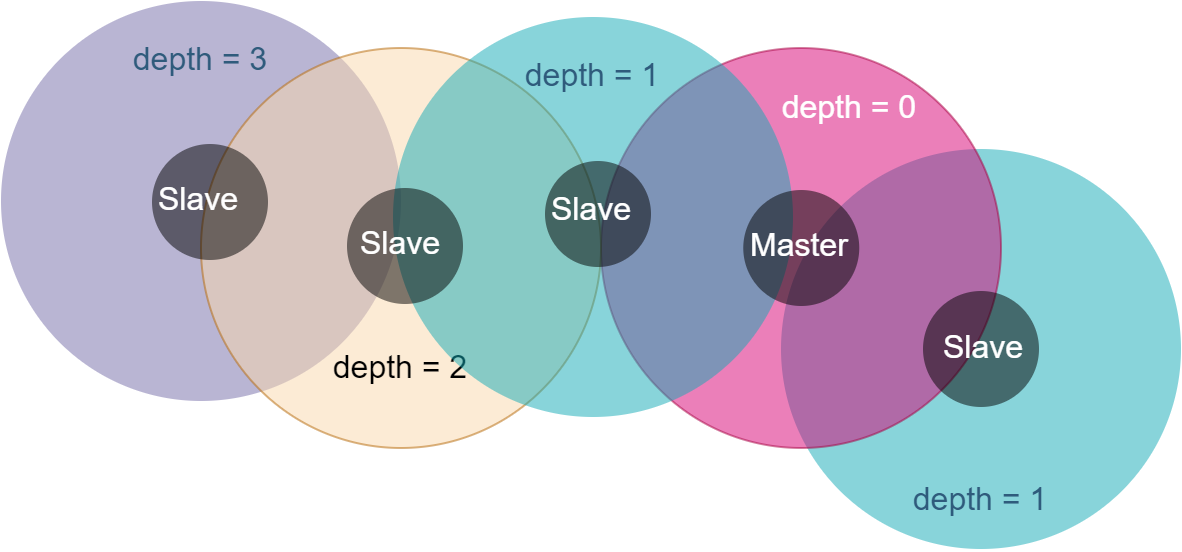
\includegraphics[width=0.8\textwidth]{Control_Hops.png}
		\caption{Konzept des Depth-Feld beim versenden einer Control-Message}\label{fig:ControlMessagesHops}
	\end{figure}

	Abbildung \ref{fig:ControlMessagesHops} zeigt die Verbreitung einer Controll-Message mithilfe des Depth-Feldes. \\
	
	\item \textit{div.} \textbf{Control-Paramter} Die restlichen Felder sind Parameter, welche den Zustand des Nodes verändern oder Parameter übergeben. 
\end{itemize}


Ein Teilnehmer signalisiert über aufblinken der grünen-LED seine Bereitschaft um weiter Control~-~Messages verarbeiten zu können. Blinkt die blaue-LED auf zeigt dies an das der Teilnehmer eine Zustands- oder Parameteränderung erhalten hat. 

Das abfragen von Control-Messages erfolgt durch Pollen. Dies hat den Ursprung, das nicht bei allen SDKs der Interrupt des Radio-Interfaces frei ist.


Der Source Code ist zur genaueren Untersuchung online\footnotemark\ verfügbar. 

\footnotetext{\url{https://github.com/Rouben94/P6_Software/blob/master/SharedLib/bm_control.c} \cite{rouben94_sharedlib_cotrol_software_git_2020}}

\subsubsection{Report}\label{subsubsec:Report}

Wie bereits in Abschnitt \ref{subsubsec:StatemachineSoftware} beschrieben werden vom Master anfragen an einen Slave getätigt um dessen Reports einzuholen. Dazu wird eine Control-Message vom Master initiiert um den Slave in den Reporting Zustand zu versetzten. Diese Nachricht wird zwar Relayed, jedoch funktioniert das anschliessende Reporting nur über eine direkte Verbindung.

Das Reporting teilt sich in eine Subscribe und Publish-Funktion auf. Der Master Subcribed auf Reports und sendet Reports-Requests an den Slave. Der Slave erwartet in der Publish-Funktion Report-Requests des Masters. Erhält ein Slave einen Request, so sendet er darufhin dem Master den verlangten Eintrag dem Master zu.

\begin{figure}[H]
	\centering
	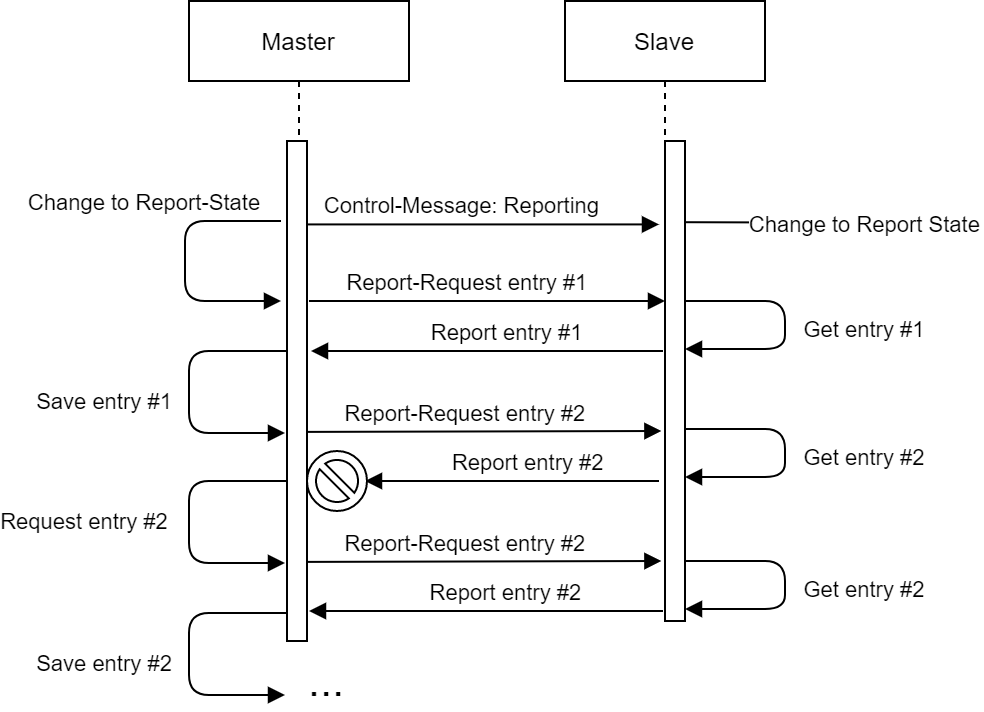
\includegraphics[width=0.9\textwidth]{Reporting_Flowchart.png}
	\caption{Ablauf des Reportings mit Handshake zwischen Master und Slave}\label{fig:ReportingAblauf}
\end{figure}

Die Abbildung \ref{fig:ReportingAblauf} zeigt den Ablauf des Reportings beispielhaft. Durch das Handshake verfahren, wie bereits in Abschnitt \ref{subsubsec:StatemachineSoftware} beschrieben, wird der Repoert-Entry 2 nochmals angefordert, da dieser nicht erfolgreich beim Master angekommen ist.

Sobald der Report als nicht mehr gültig erkannt wird, wird das Reporting beidseitig beendet. Dies geschieht durch prüfen des Zeitstempel-Feld des jeweiligen Report Eintrages auf null. Falls keine Verbindung zustande kommt, brechen Master, sowie Slave nach einer bestimmten Anzahl von Versuchen das Reporting ab.

Der Source Code ist zur genaueren Untersuchung online\footnotemark\ verfügbar. 

\footnotetext{\url{https://github.com/Rouben94/P6_Software/blob/master/SharedLib/bm_report.c} \cite{rouben94_sharedlib_report_software_git_2020}}

\subsubsection{Logging}\label{subsubsec:Logging}

Das Logging-Modul ist für das verwalten der Log-Daten im RAM sowie im FLASH zuständig. Es definiert das Format eines Log-Eintrages, welcher bereits in Abschnitt \ref{subsubsec:Messgrössen} vorgestellt wurde. Die Länge eines Eintrages setzt sich zu 28-Bytes zusammen. Zudem beherbergt dieses Modul die gesamten Log-Daten als Array von 3000 Log-Einträgen. Diese konstante kommt folgendermassen zustande. Pro Client können maximal 1000 Nachrichten verschickt werden. Ein Server soll mit maximal drei Clients in der sleben Gruppe sein. Damit er alle Einträge aufnehmen kann, wurde die Länge des Arrays auf 3000 festgelegt. Somit müssen 84kByte RAM und Flash für das Log zur Verfügung stehen. Die im Ablauf benötigten Funktionen des Moduls lassen sich folgendermassen beschreiben. 

\begin{itemize}
	\item \textit{\textbf{bm\_log\_clear\_ram()}} Wird genutzt um alle Log-Einträge aus dem RAM zu entfernen.
	\item \textit{\textbf{bm\_log\_append\_ram()}} Fügt einen Log-Eintrag dem RAM hinzu. Das Modul verwaltet selbst den nächsten freien Index. 
	\item \textit{\textbf{bm\_log\_clear\_flash()}} Bewirkt ein löschen des gesamten Logs im FLASH. 
	\item \textit{\textbf{bm\_log\_save\_to\_flash()}} Schreibt den gesamten Log vom RAM in das FLASH. 
	\item \textit{\textbf{bm\_log\_load\_from\_flash()}} Lädt den gesamten Log vom FLASH in das RAM. 
	\item \textit{\textbf{bm\_log\_init()}} Initialisiert das Logging-Modul.
\end{itemize} 

Die Abarbeitung des Flash Moduls wurde bei der Zephyr direkt in diesem Log-Modul integriert. Handelt es sich um eine nRF-SDK findet die behandlung des Flashs in einem separaten Modul statt (siehe Abschnitt \ref{subsubsec:FlashSave}).

Zephyr organisiert die Flash-Bereiche mithilfe eines Device-Tree-Source-Files (DTS). Darin werden verschiedene Partitionen definiert. Die Partition in welchen die Daten gespeichert werden, ist vom Bootloader für ein DFU-Upgrade reserviert. Sofern kein DFU-Upgrade im gang ist kann der Bereich beliebig genutzt werden. Die Partition muss mindestens 84kByte zur Verfügung Stellen. Der Zugriff auf das Flash ist über das Zephyr OS geregelt, welches einen Flash-Driver zur Verfügung stellt. Dieser kann eine Pages-Grösse von 4kByte löschen. 

Der Source Code ist zur genaueren Untersuchung online\footnotemark\ verfügbar. 

\footnotetext{\url{https://github.com/Rouben94/P6_Software/blob/master/SharedLib/bm_log.c} \cite{rouben94_sharedlib_log_software_git_2020}}

\subsubsection{Flash Save}\label{subsubsec:FlashSave}

Mittels diesem Modul wird das abspeichern von Daten aus dem RAM in das FLASH mithilfe der Flash-Device-Storage (FDS) API behandelt. Dies ist eine API, welche in der \textit{nRF SDK for Mesh}, sowie in der \textit{nRF SDK for Thread and Zigbee} angeboten wird. Sie erlaubt das abspeichern von Daten im Flash und implementiert ein \textit{Basic-Wearleveling}. \\

Das FDS-Modul beginnt, falls nicht anders vorgesehen, direkt unterhalb der Bootloader-Adresse mit dem abspeichern der Daten im Flash. Mittels der \textit{sdk-config.h} Konfiguration werden die Länge des Flash-Bereichs und weitere Einstellungen für das FDS-Modul festgelegt. Die abzuspeichernden Daten werden in Records unterteilt. Zur Abspeicherung der Log-Daten wurde nur ein Record verwendet. \cite{nordic_semi_nrf5_sdk_flash_data_storage_2020}

Der Source Code ist zur genaueren Untersuchung online\footnotemark\ verfügbar. 

\footnotetext{\url{https://github.com/Rouben94/P6_Software/blob/master/SharedLib/bm_flash_save.c} \cite{rouben94_sharedlib_flash_save_software_git_2020}}

\subsubsection{CLI}\label{subsubsec:CLI}

Mit diesem Modul werden Ein- / Ausgaben über das Command-Line-Interface (CLI) ermöglicht. Die wohl einfachste Funktionalität ist das ausgeben über einen Log-Befehl. Dieser ist mittels \textit{bm\_cli\_log("Hello")} aufrufbar. Dieses Kommando wird auf die jeweilige Umgebung (SDK) angepasst. Bei der \textit{nRF SDK} werden Logs mittels dem \textit{NRF\_LOG()} Befehl, bei \textit{Zephyr} mithilfe von \textit{printk()} ausgegeben.

Die zentrale Funktionalität des Moduls bezieht sich auf das verarbeiten von CLI-Befehlen. Dafür werden verschiedene CLI-Befehlssätze angeboten, welche im Sub-Modul \textit{bm\_cli\_cmds.c} defniert sind. 

\begin{itemize}
	\item \textit{\textbf{setNodeSettings}} Mithilfe dieses Befehlssatzes können die Einstellungen eines Slaves (Server/Clients) geändert werden. Eine Beispielhafte Eingabe könnte folgendes Format aufweisen. 
	\textit{setNodeSettings <MAC in Integer format> <GroupNumber> <Node Id> <Ack> <AdditionalPayloadSize> <BenchmarkTrafficGenMode> <DST\_MAC\_1> \linebreak <DST\_MAC\_2> <DST\_MAC\_3>}. Die Bedeutung der einzelnen Felder sind in Abschnitt \ref{MeshBenchmarkKonzeptundTestumgebung} angedeutet.
	\item \textit{\textbf{getNodeReport}} Mithilfe dieses Befehlssatzes können die Reports eines Slaves (Server/Clients) abgefragt werden. Eine Beispielhafte Eingabe könnte folgendes Format aufweisen. 
	\textit{getNodeReport <MAC in Integer format>}. Die Bedeutung der einzelnen Felder sind in Abschnitt \ref{subsubsec:NodeIdentification} angedeutet. 
	\item \textit{\textbf{startBM}} Mithilfe dieses Befehlssatzes wird ein Benchmark gestartet. Eine Beispielhafte Eingabe könnte folgendes Format aufweisen. 
	\textit{startBM <BenchmarkTime (seconds)> <BenchmarkPacketsCount>}. Das erste Feld gibt die Benchmark Zeit in Sekunden an. Beim zweiten Feld handelt es sich um die Anzahl Nachrichten, welche versendet werden sollen. 
\end{itemize}

Erhält der Master eine der oben erwähnten Befehlssätze und löst eine darauffolgende Control-Message aus. Die zugewiesenen Paramter werden ebenfalls mithilfe des Moduls abgespeichert und initialisiert. 

Der Source Code ist zur genaueren Untersuchung online\footnotemark\ verfügbar. 

\footnotetext{\url{https://github.com/Rouben94/P6_Software/blob/master/SharedLib/bm_cli.c} \cite{rouben94_sharedlib_cli_software_git_2020}}

\subsubsection{Traffic Generator}\label{subsubsec:TrafficGenerator}

Im folgenden Modul werden die Sende-Zeitwerte von Nachrichten generiert. Das Konzept dazu wurde bereits in Abschnitt \ref{subsec:TrafficGeneration} erläutert. Dabei wird zwischen zufälligen und sequentiellen Werten unterschieden.  \\

Wird eine Messung mit sequentiellen Werten gestartet erstellt dieses Modul, abhängig von den Benchmark-Parametern, eine Abfolge gemäss der bereits erwähnten Formel \ref{eq:TrafficGenerationSeq}. \\

Wird eine Messung mit zufälligen Werten gestartet erstellt dieses Modul, abhängig von den Benchmark-Parametern, eine neu generiertes Set oder verwendet ein bereits vorhandenes Set an zufälligen  Werten. Es existieren 25 verschiedene vordefinierte Sets. Diese wurden vorgängig mittels der Webseite \textit{random.org} erzeugt. Die Einstellungen, welche zur Erzeugung der Werte verwendet wurden, sind im Anhang \ref{app:RandomTrafficGeneration} zu finden. \\

Wurde ein Set festgelegt werden diese Werte mittels eines \textit{Bubble-Sort} Algorithmus in aufsteigender Reihenfolge sortiert. Anschliessend müssen die Werte auf den Zeitbereich des Benchmarks skaliert werden. Da es isch bei den zufällig generierten Werten um uInt16-Datentypen handelt liegt der Wertebereich zwischen 0-65535. Die Werte werden gemäss Formel \ref{eq:TrafficGenerationRand} berechnet. 

\begin{equation}\label{eq:TrafficGenerationRand}
T_{Msg\_send} =  \frac{V_{Rand}}{UINT16MAX} \cdot T_{Benchmark}
\end{equation}

\begin{small}
	\begin{center}
		\begin{tabular}{ll}
			$T_{Msg\_send}$ & Zeitpunkt zu welchem die Nachricht gesendet wird.\\
			$T_{Benchmark}$ & Benchmark Dauer (siehe \ref{tab:ParameterBenchmarkMessreihe})\\
			$V_{Rand}$ & Random Value aus dem Set \\
			$UINT16MAX$ & Maximaler Wert des UInt16 (65535) \\
		\end{tabular}
	\end{center}
\end{small}

\footnotetext{\url{https://github.com/Rouben94/P6_Software/blob/master/SharedLib/bm_rand.c} \cite{rouben94_sharedlib_rand_software_git_2020}}

\subsubsection{Low Level Radio}\label{subsubsec:LowLevelRadio}

Der Low-Level-Radio Treiber soll möglichst unabhängig direkt mit dem Radio-Interface operieren. Er stellt die für das Verwalten der Messung notwendigen Funktionen zur Verfügung. Senden oder Empfangen von Daten sollen mittels einfachen Aufrufen möglich sein.

Das Radio-Interface wird fast identisch zur P2P-Testinfrastruktur bedient (siehe Abschnitt \ref{sec:LowLevelRadioDriver}). Lediglich auf das verwenden von Interrupts musste verzichtet werden, da die Meisten Radio-Driver der Mesh-Stacks diese bereits belegten. Insbesondere beim Zephyr findet die Initialisierung des Radio-Treiber vor dem Aufrufen der Statemachine statt. Somit wurden die Events durch pollen abgewartet.

Der Source Code ist zur genaueren Untersuchung online\footnotemark\ verfügbar. 

\footnotetext{\url{https://github.com/Rouben94/P6_Software/blob/master/SharedLib/bm_radio.c} \cite{rouben94_sharedlib_radio_software_git_2020}}

\subsection{Benchmark Management}\label{subsec:Benchmark Management}

Um die Verwaltung einer Messung zu automatisieren dienen folgende Python-Scripts. Die Scripts werden auf der BMS (Benchmark Managment Station) ausgeführt. Die Konfiguration der Teilnehmer wird mittels einem Excel-File durchgeführt (siehe Abschnitt \ref{subsubsec:NodeConfiguration}). 


\subsubsection{Flasher}\label{subsubsec:Flash}

Dieses Script dient dazu alle nRF52-Dongles mit der entsprechenden Firmware zu flashen. Dazu liest das Script die Konfigurationsdatei aus. Mithilfe der dort vorhanden Informationen fordert das Script den Benutzer dazu auf die entsprechende Dongle-Nummer einzustecken. Sobald der Dongle eingesteckt wurde beginnt das Script mit dem Flashen. Dies geschieht mittels dem nrfutil-Tool. 

\subsubsection{Configurator}\label{subsubsec:Configurator}

Mithilfe des Configurator-Scripts kann eine voreingestellte Konfiguration auf die einzelnen Teilnehmer verteilt werden. Das Script arbeitet die Konfigurations-Einträge der Reihe nach ab. Mittels dem an der BMS angeschlossenen Masters sendet das Script den entsprechenden Konfigurationsbefehl ab. 

\subsubsection{Benchmark and Reporter}\label{subsubsec:BenchmarkandReporter}

Über dieses Script wird entweder eine Messung gestartet oder die Resultate einer vorhergehenden Messung einzuholen. Wird eine neuer Benchmark initiiert muss der Benutzer die Benchmark-Parameter angeben. Anschliessend startet das Script über den angeschlossenen Master den Vorgang. Während der Messung zeigt das Script die Meldungen des Masters an.

Nach beenden der Messung können die Reports mithilfe des Scripts eingeholt werden. Dazu fordert das Script den Benutzer auf sich in die nähe des ersten Slaves zu begeben. Nach dem Bestätigen fängt das Script an die Daten des Slaves einzusammeln. Nach einsammeln aller Daten der Slaves schreibt das Script die Werte in ein CSV-File. 

\subsubsection{Analysis}\label{subsubsec:Analysis}

Sind alle Report-Daten in einem Excel-File abgespeichert, können die Messgrössen mithilfe des Analysis-Scripts berechnet werden. Dieses wertet die einzelnen Daten aus und gibt die Messdaten in einem ergänzenden CSV-File zur Verfügung. Dieses Script wird nicht länger benötigt da die Auswertung neu komplet in Excel erfolgt. 

